\chapter{Results}

A set of ligands from PDBbind has been downloaded and used for testing
purposes (common core construction as well as mutation routes). It
should be noted, however, that the common core of pairs of these ligands
in some cases violate the rules of Transformato concerning a valid
maximum common substructure, i.e. dummy regions are connected by more
than one atom to the common core (which basically implies that the
atom is part of a ring structure). 

In the current implementation of the mutation algorithm this problem
is solved by a helper function which chooses one of the possible connections
between one of the atoms to the common core. For the following processing
of the mutation algorithm, this connection is arbitrarily distinguished
and the other ones removed. 

...

\section{Visualizations}

The mutation route can be visualized using a color gradient (additionally
to numbering, see figures above).

Py3dMol is used for a 3D-animation of the mutation process. Fig. 5.1
shows two molecules and their shared common core.

\begin{figure}
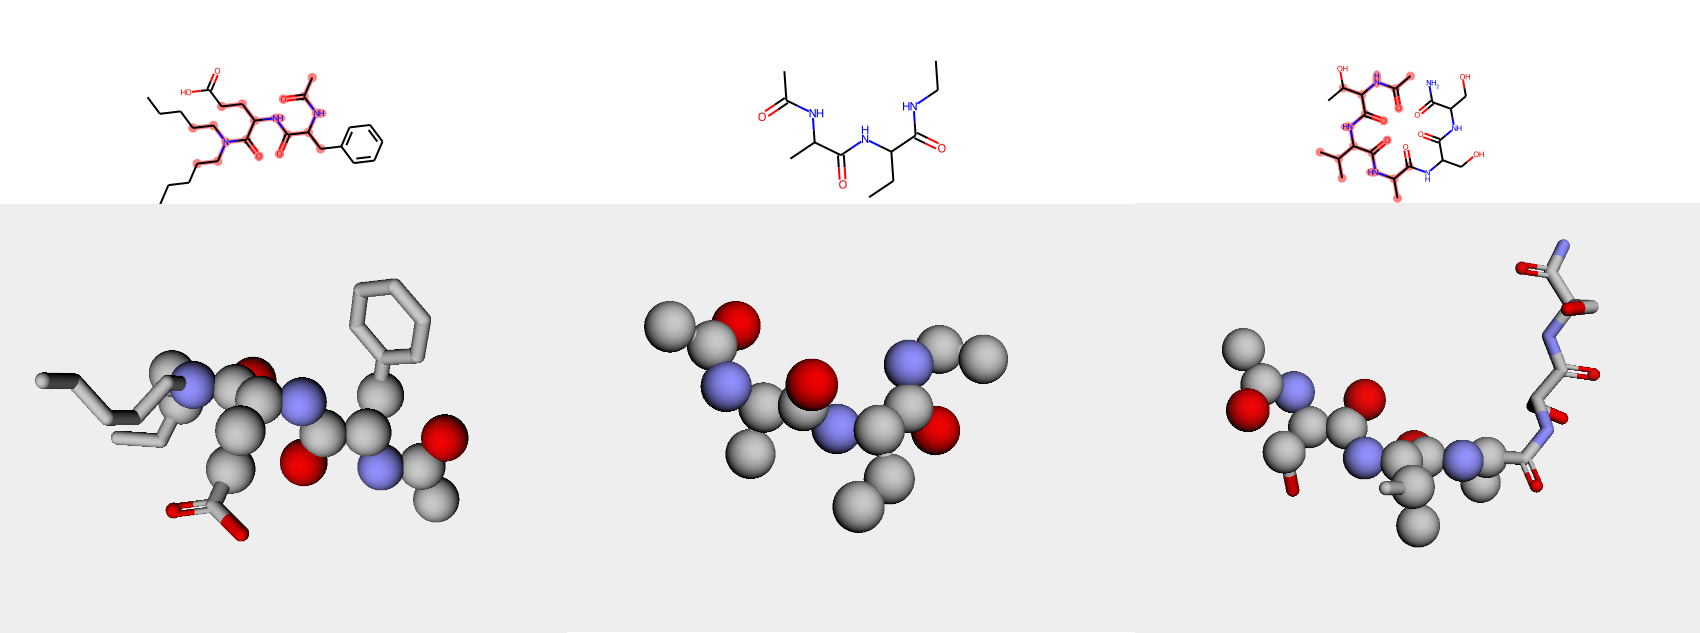
\includegraphics{trafo_py3d_1verkleinert}

\caption{Visualization of the mutation route using py3dmol; upper row: rdkit-representations
of both molecules and the common core; lower row: py3Dmol visualizations;
left and right: molecules; middle: common core of both molecules}

\end{figure}

